% THIS IS SIGPROC-SP.TEX - VERSION 3.1
% WORKS WITH V3.2SP OF ACM_PROC_ARTICLE-SP.CLS
% APRIL 2009
%
% It is an example file showing how to use the 'acm_proc_article-sp.cls' V3.2SP
% LaTeX2e document class file for Conference Proceedings submissions.
% ----------------------------------------------------------------------------------------------------------------
% This .tex file (and associated .cls V3.2SP) *DOES NOT* produce:
%       1) The Permission Statement
%       2) The Conference (location) Info information
%       3) The Copyright Line with ACM data
%       4) Page numbering
% ---------------------------------------------------------------------------------------------------------------
% It is an example which *does* use the .bib file (from which the .bbl file
% is produced).
% REMEMBER HOWEVER: After having produced the .bbl file,
% and prior to final submission,
% you need to 'insert'  your .bbl file into your source .tex file so as to provide
% ONE 'self-contained' source file.
%
% Questions regarding SIGS should be sent to
% Adrienne Griscti ---> griscti@acm.org
%
% Questions/suggestions regarding the guidelines, .tex and .cls files, etc. to
% Gerald Murray ---> murray@hq.acm.org
%
% For tracking purposes - this is V3.1SP - APRIL 2009

\documentclass{acm_proc_article-sp}

\begin{document}

\title{Prefetching for linked data structure}

%\subtitle{[Extended Abstract]
%\titlenote{A full version of this paper is available as
%\textit{Author's Guide to Preparing ACM SIG Proceedings Using
%\LaTeX$2_\epsilon$\ and BibTeX} at
%\texttt{www.acm.org/eaddress.htm}}}
%
% You need the command \numberofauthors to handle the 'placement
% and alignment' of the authors beneath the title.
%
% For aesthetic reasons, we recommend 'three authors at a time'
% i.e. three 'name/affiliation blocks' be placed beneath the title.
%
% NOTE: You are NOT restricted in how many 'rows' of
% "name/affiliations" may appear. We just ask that you restrict
% the number of 'columns' to three.
%
% Because of the available 'opening page real-estate'
% we ask you to refrain from putting more than six authors
% (two rows with three columns) beneath the article title.
% More than six makes the first-page appear very cluttered indeed.
%
% Use the \alignauthor commands to handle the names
% and affiliations for an 'aesthetic maximum' of six authors.
% Add names, affiliations, addresses for
% the seventh etc. author(s) as the argument for the
% \additionalauthors command.
% These 'additional authors' will be output/set for you
% without further effort on your part as the last section in
% the body of your article BEFORE References or any Appendices.

\numberofauthors{1} %  in this sample file, there are a *total*
% of EIGHT authors. SIX appear on the 'first-page' (for formatting
% reasons) and the remaining two appear in the \additionalauthors section.
%
\author{
% You can go ahead and credit any number of authors here,
% e.g. one 'row of three' or two rows (consisting of one row of three
% and a second row of one, two or three).
%
% The command \alignauthor (no curly braces needed) should
% precede each author name, affiliation/snail-mail address and
% e-mail address. Additionally, tag each line of
% affiliation/address with \affaddr, and tag the
% e-mail address with \email.
%
% 1st. author
\alignauthor
Liang Yan \\%\titlenote{Dr.~Trovato insisted his name be first.}\\
       \affaddr{Dept. of Computer Science}\\
       \affaddr{Univ. of Michigan Tech, Houghton}\\
       \email{liayan@mtu.edu}
% 2nd. author
%\alignauthor
%Soner Onder\\%%\titlenote{The secretary disavows
%any knowledge of this author's actions.}\\
%       \affaddr{Dept. of Computer Science}\\
%       \affaddr{Univ. of Michigan Tech, Houghton}\\
%       \email{soner@mtu.edu}
}

% There's nothing stopping you putting the seventh, eighth, etc.
% author on the opening page (as the 'third row') but we ask,
% for aesthetic reasons that you place these 'additional authors'
% in the \additional authors block, viz.
%\additionalauthors{Additional authors: John Smith (The Th{\o}rv{\"a}ld Group,
%email: {\texttt{jsmith@affiliation.org}}) and Julius P.~Kumquat
%(The Kumquat Consortium, email: {\texttt{jpkumquat@consortium.net}}).}
%\date{30 July 1999}
% Just remember to make sure that the TOTAL number of authors
% is the number that will appear on the first page PLUS the
% number that will appear in the \additionalauthors section.
\maketitle

\begin{abstract}
As the performance gap of CPU and memory continues to grow, hiding memory
latency are becoming more and more important for a high performamce
computer system. Prefetching is taken to be an effictive method to decrease
memory dependence compared to multithreading. In array-based data
structure program prefetching 
already gets a good performance. However, prefetching for linked data
structure (LDS) is still difficult because separate dynamically
allocated objects are disjoint, and the access patterns are less
regular and predictable.

In this paper, we focus on the research based on LDS, and
classify the research method into four different directions,
chase-pointer based on 
the successive layout of the LDS, jump-pointer based on thenon-consecutive
layout of the LDS, 
content directed prefetching(CDP) based on the memory block, prefetching
from the momory side. 

All of these approachs offer an good performance
to hide memory latency than base system without prefetching technique,
a cooperate approach combined Jump-Pointer software and Chase-Pointer
hardware implementation make an impressive result during the data
analysis approach. Although CDP approach only does well for part of
applications , its simple idea and hardware implementation still leave
a huge development space. Memory side prefetching becomes available
as the showing up of processor in memory (PIM), and gives a better
parallelism implementation.   
\end{abstract}

% A category with the (minimum) three required fields
%\category{H.4}{Information Systems Applications}{Miscellaneous}
%A category including the fourth, optional field follows...
%\category{D.2.8}{Software Engineering}{Metrics}[complexity measures, performance measures]
%\terms{Theory}
%\keywords{ACM proceedings, \LaTeX, text tagging} % NOT required for Proceedings

\section{Introduction}

According to Figure 1,we could find that  microprocessor
performance has improved 60\% per year, while memory access time has improved
only 10\% per year since 1980.\cite{Yang:2002:PMH:646349.690705} The
performance gap of  Memory and high performance CPU makes memory
latency an improtant performance bottleneck today. 
\begin{figure}
\centering
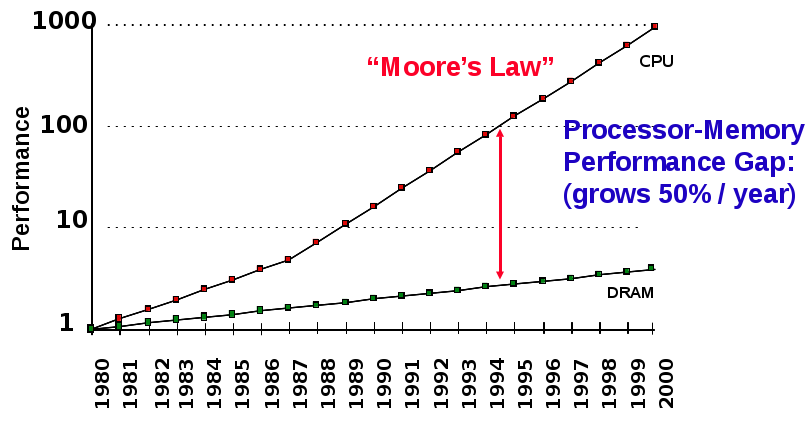
\epsfig{file=memory.png,height=1.6in, width=2.8in}
\caption{Memory latency.}
\end{figure}

Memory latency includes two different ones. First is store latency, to
save some values to the memory, The other one is load 
latency, to read some values from the momory. Write latency
is not a big problem,because we can use buffer and pipeline techniques to hide
it. However, read latency is much more difficult to avoid, it requires
to decouple the request for data from the use of that data. There are two
main techniques for tolerating read latency are
prefetching  and multithreading
\cite{Luk:1996:CPR:248208.237190}. Prefetching works by accessing
memory earlier than demand 
fetching a cache block when a cache miss occurs. In contrast,
multithreading  switches from one concurrent
thread to another upon a cache miss. 

Multithreading is very popular among the modern high-performance
processor, however prefetching we are talking in this parper is still
an important approach. Comparing to multithreading, prefetch do not
need to find out enough independent instruction which is very hard in
real program, also, it does not need to change thread context which is a high
cost in modern processor. 

Prefetching works very well for programs with regular access
patterns(e.g.,array), there are already some research on this
approach, whether using software,hardware,or hybrid techniques. 
Unfortunately, many applications create sophisticated data
structures using pointers, which are called linked data structure in
this paper, and do not exhibit sufficient regularity
for conventional prefetch techniques to exploit. This is also the
reason we choose it to be the topic of this paper. 
\cite{Vanderwiel:2000:DPM:358923.358939}
\subsection{An Overview}

In this paper, we focus on the prefetching approach for Linked data
structure, the rest of the work is organized as follows. First, In
Section 2, we analysis why prefetching LDS is difficult, and make a
classification for the approach dealing with this problem then
introduce the evaluation framework for this data structure.  In
Section 3-6, we start introduce the implementation for different
approachs, give a brief evaluation to anlysis the advantage and
disadvantage of each Implementation. In
Section 7, we will introduce some other related 
research work which made some improvement for the approach in Section
3-6, then offer our survey conclusion in Section 8 finally.

\section{Background}

\subsection{Linked data structure}

Linked data structures (LDS) such as lists and trees are used in
many important applications. The importance of LDS is growing
with the increasing popularity of object oriented language C++, Java,
and other database systems that use linked object graphs and function tables. 
\cite{Vanderwiel:2000:DPM:358923.358939}

According to Figure 2, we could see the difference of Linked data
structure and Array clearly. Array address are continuous,
we could  access an array reference A[i] once we know the offset
i. However,  we could not access p->next unless we know the value stored in p. 
This difference makes more challenging to prefetch LDSs than arrays.

\begin{figure}
\centering
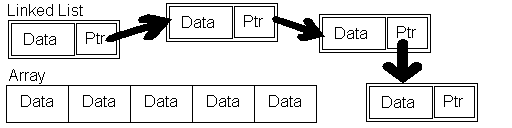
\epsfig{file=linklist.png,height=0.8in, width=2.6in}
\caption{Linked list and Array}
\end{figure}

\subsection{Reasearch classification}

According to the implementation, prefetching could be divided into
softeware-based and hardware-based approaches,  
either way has its advantage and
disadvantage.\cite{Chen:1994:PSS:192007.192030}  
Hardware-based prefetching  requires some extra unit connected to
the cache but little modification to the processor. The main advantage is that
prefetching are dynamicly at run-time without compiler intervention. The
drawbacks are more Hardware resources more money cost and energy cost.
In contrast, software-directed approaches 
rely on compiler technology to do static progmm analysis 
and to selectively insert prefetch instructions.
The drawbacks are that there is some non-negligible
execution overhead due to the extra prefetch instructions and 
that some useful prefetchilng cannot be uncovered at run-time.
\cite{Guo:2011:EHD:1993125.1993134}\cite{Baer:1995:EHD:626514.627012}

Recently, prefetching has been taken an effective approache to tolerate these 
large memory latencies, researchers have begun investigating prefetching
techniques for LDS traversal problem using four different
approaches.\cite{Harrison:1996:EMA:237578.237595}  

Techniques in the first approach, Chase-Pointer prefetching,
it only prefetch pointer chains sequentially using the natural
pointers belonging 
to the LDS.\cite{Luk:1996:CPR:248208.237190}
\cite{Roth:1998:DBP:384265.291034}\cite{Choi:2004:GFP:986533.986536} 

Techniques in the second approach, which we call
jump pointer techniques, insert additional pointers into the LDS
to connect non-consecutive link elements.\cite{Roth:1999:EJP:307338.300989}
\cite{Collins:2002:PCA:774861.774869}\cite{824351}
These jump pointers allow prefetch instructions to get link
elements further than the chain pointer without sequentially
traversing the intermediate links. 

Cooksey.et.al and Ebrahimi.et.al provided a new approach, they did not
make prediction by analysising the data flow of the pointer, instead,
they mointered the momeory traffic at a memory block, Cooksey
pointed out that there is a strong relationship between the load address
used currently with the load address will be used in future. Ebrhimi's
ECDP approach improved Cooksey's implementation by adding a new
concept pointer groups. 
\cite{Cooksey:2002:SCD:635506.605427}\cite{4798232}

At last, Young.et.al developed a push model, which was different from
the oringinal pull model, He pointed out that most of the prefetch
request were start from the processor first and then pull the
prediction data out of memory, however his idea was using a prefeth
mechanism to dectect the future pointer and push it directly to the
processor, his most work is based on a microarchitecture platform,
Hughes.et.al put this idea to a multi-PIM(processor in memory) system
with a current state-of-the-art processor integrated with DRAM on the PIM.
\cite{Yang:2002:PMH:646349.690705}\cite{Hughes:2005:MPL:1066486.1066491}

\begin{figure*}
\centering
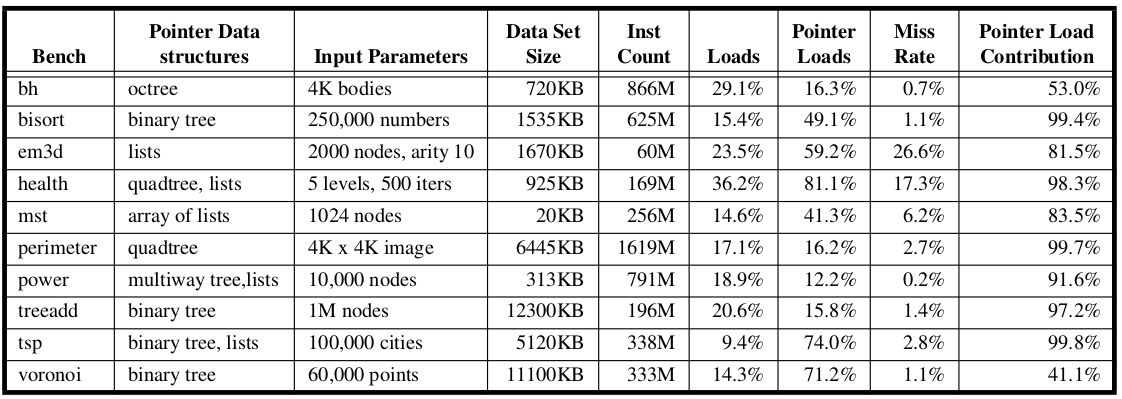
\epsfig{file=olden.PNG,height=2in, width=5in}
\caption{Olden Benchmark}
\end{figure*}

\subsection{Evaluation Benchmark }

To measure a technique if it hides memory latency when accessing LDS well,
we need to have a spacial benchmark, and the benchmark must have 
a good property on LDS, also we need to know this benchmark very
well. We need to know how many LDS access in the program, we aslo need
to know how much part it take in this whole problem, the Olden
benchmark suite designed by Rogers becomes a good choice
here.\cite{Rogers:1995:SDD:201059.201065}  

The Olden benchmark suite includes different kinds of LDS code, 
bh and em3d which are small and medium sized scientific codes, health
and power which are process simulations programms, mst and tst
implements the graph optimization routines, performance and voroni as
the graphics utilities,bisort, a sorting routine and a toy tree
benchmark treeadd.Figure 3 gives a detail analysis form  the summary of the
benchmarks, the sizes and types of linked data structures used, input
parameters and dynamic instruction counts.  

\section{Chase-Pointer Prefetching}

Luk et al. pointed out prefetching LDS should include two major
phases, analysis phase and schedule phase. When doing prefetch
we need to predict which memory reference are likely to make a
cache misss in analysis phase, and we also need to
insert the prefetch as close as possible to hide the momory latency
efficiently in the schedule phase. 
The schedule phase is more difficult to fulfill and it  determins most
of the prefetching effiency .\cite{Luk:1996:CPR:248208.237190}Most
prefetching approach focus on how to make the schedule phase better. 
 
He also provided a formular for Pointer-chasing Problem here.
At a LDS node $n_i$ with address $A_i$, and wish to prefetch the node
$n_{i+d}$ which will visited d nodes after $n_i$, d should be just
large enough to hide the cache miss latency, $d=\frac{x}{y}$, L is the
expected miss latency and W is the estimated amount of computation
between node access in cycles. To prefetch $n_{i+d}$, we must need to
know its address $A_{i+d}$, The relationship between $A_{i+d}$ and
$A_{i}$ should be : 
\begin{displaymath}
A_{i+d}= \mathcal{F}(d,A_i)
\end{displaymath}
To overcome the pointer-chasing problem, $||\mathcal{F}||$ should be
as small as possible.

\subsection{Greedy Prefetching}

\subsubsection{Basic Idea}

Greedy Prefetching is a basic algorithm for pointer-chasing problem.
Its basic idea is that the distance we prefetch should not be lower than
its real used node, For example, if we prefeth p->next->next, the
distance is 2, but real used is work(p->next->next->next->next), the
distance is 4, then prefeth does not hide the momeory latency
fully. We need to do prefeth twice to cover the whole memory latency.
The idea situation should let both equal to each other.

\begin{figure}
\centering
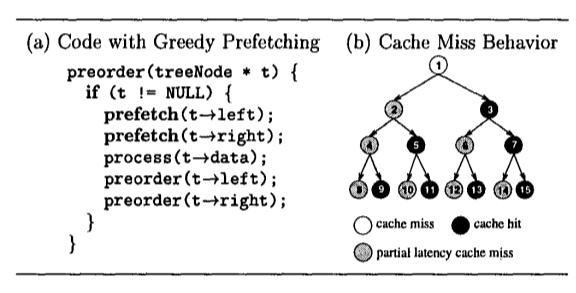
\epsfig{file=greedy.PNG,height=1.8in, width=3in}
\caption{Greedy Prefetching}
\end{figure}

\subsubsection{Implementation}

We use the binary tree example in Luk's paper to illustrate  how greedy
prefetching works.\cite{Luk:1996:CPR:248208.237190} 
From Figure 4(a), there are two children for the binary tree, so the
greedy prefetching needs to prefetch the two child nodes to hide
the fully latency. Figure 4(b) shows the caching behavior of each node. 
There is a assumption that function process() will take half cache
miss latency. so when goes to process() after prefetching left and
right child node, it always loose the left child which is the half
cache latency, also the root node is a cache miss too because no
prefetch for the first step, then the greedy algorith here hides all
right child node in this binary three and covered 50\% latency.  

\subsubsection{Evaluation}

Even the greedy prefetching does not offer precise control over the
prefetching distance which will cause unnecessary cache pollution, it
still hase some obvious advantages: (1) all prefeth points are natura
point in the LDSs, then no additional storage and computation; (2)
It is very easy to make an application in compiler; (3) It could be
used for almost applications since its simple. So Greedy prefetching
is widely used in prefetching techniques today.

\subsection{Dependence Based Prefetching}

Recent work \cite{Onder:2002:CEM:645989.674303} has
demonstrates that memory dependence prediction is an effective technique
since it allows issuing of the load instructions early.
These studies have focused primarily on memory dependences when
stores and loads accessing to the same location. 

According to Section 1, we know that prefetch is more responsible for
read latency, Roth.et.al provided a technique which useing load value
dependences, a 
class of dependences between loads that produce addresses and those that consume
those addresses. He pointed tht load value dependences capture 
regularities in the address generation process rather than in the
addresses themselves.\cite{Roth:1998:DBP:384265.291034}

\begin{figure}
\centering
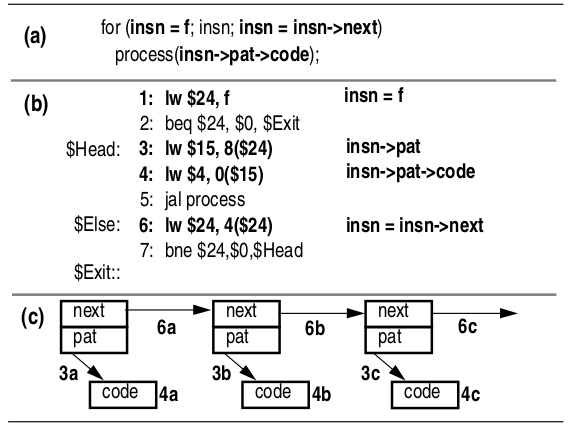
\epsfig{file=dependence.png,height=2in, width=3in}
\caption{LDS traversal example. (a) Source and (b) machine
code that traverses a linked list. (c) List layout in memory.}
\end{figure}

\subsubsection{Pointer-load classification}
Roth.et.al made a classification for pointer loads
here,\cite{Roth:1998:DBP:384265.291034} He divided 
the load type into recurrent,traversal, and data loads. 

Recurrent loads are the loads that they will produce the address
will be consumed by themselves in the future. For example, p->next,and
the next time it is still uses p->next, like p->next->next, then this
is recurrent loads. However if it dose not use p->next next time, like
p->next->data, then it becomes traversal loads. It is very easy to
understand data load, not like recurrent loads and traverse loads
which produce address for next time, data load only saves data value. 

According to the definitions, we could easily find different loads in
Figure 5, Instruction 6, which loads the next field of an element,
is a recurrent load. Instruction 3 loads the address of the pat
structure and is a traversal load. Instruction 4 loads the code field and
is a data load. 

\subsubsection{Hardware Implementation}
After Roth.et.al providing the load pointer classification scheme, they
designed a hardware mechanism. 
\begin{figure}
\centering
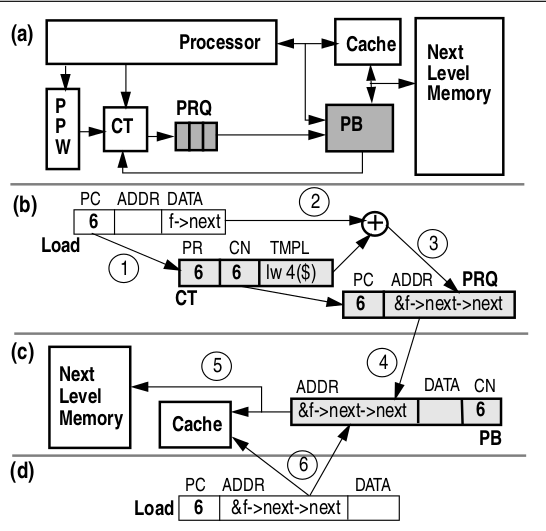
\epsfig{file=dep-hard.png,height=3in, width=3in}
\caption{Prefetch example. (a) Block schematic of the PB and
PRQ. (b) A completed load probes the CT, finds a potential
consumer and enqueues a prefetch request onto the PRQ. (c) If
a data cache port is free, the prefetch request is dequeued and
issued to the prefetch buffer. The prefetch buffer checks the first
level cache for the block, issuing a request to the second level
cache on a miss. (d) A load uses the prefetched block.}
\end{figure}

As shown in Figure 6(a), they designed several components, Correlation   
table(CT), Potential Producer Window (PPW), Prefetch Request Queue
(PRQ), and Prefetch Buffer (PB).

Correlation Table is a table with dependence information in it. The
dependence comes from two load instruction that one(PR) produces an
address and the other one(CN) uses it. It also contains an address
generation template (TMPL) in the entry. TMPL is a condensed form of
the CN, it only uses the opcode and an offset.    

Roth et al. also constructed a Potential Producer Window (PPW), which
saves a list of the most recently loaded values and the
corresponding instructions. 

They also used a Prefetch Request Queue (PRQ) buffers to prefetch
requests until data ports are available to service them. The
Prefetch Buffer (PB) is a small data cache that temporarily holds
prefetched blocks. 

Let us see how this mechanism works through the example in Figure 6.
Before start, the mechanism need to construct the CT first. The CT are
created when an load instruction is commited, it will check the commit
load instruction with PPW, if match then save it to CT, after the CT
is constructed, the prefetching begins. In action 1, when the
instruction load 6 completes, it will check the Correlation Table to
find the correlation, if so, then comes to action2, here it will
compute the prefetch address and save it on PRQ(action 3), PB as the
buffer will send the entry of PRQ to cache when data cache port is
available, it will also issue a request on next level memory(action 5)
if not find it in current data cache.

\subsubsection{Evaluation}

\begin{figure}
\centering
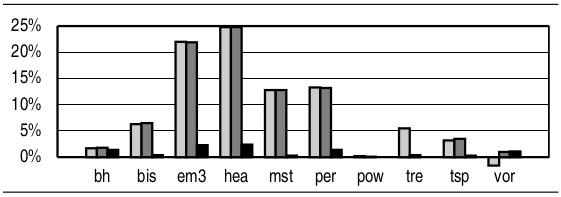
\epsfig{file=depdata.png,height=1in, width=3in}
\caption{Performance impact of dependence-based
prefetching. Speedups of dependence based prefetching
without (lt gray) and with (dk gray) a coarse confidence
scheme, compared to a system that prefetches by doubling the
line size, and thus overall size, of the data cache
(black)..\cite{Roth:1998:DBP:384265.291034}} 
\end{figure}
Roth et al. measured the impact performance  of dependence based
prefetching with three different 
prefetching scheme. The first is the one  describing
all along, the second one is augmented with a coarse confidence
mechanism that turns off prefetches if the corresponding static
load has hit in the first level data cache 8 or more times in a
row. The third scheme is a base form of prefetching, namely a system
that has twice the on-chip data cache and uses 64, rather than 32, byte lines.
These speedups are shown in as light and dark gray and dark bars, respectively
in Figure 7. The data showes that Dependence-based prefetching improves the
performance of several benchmarks significantly, except having a slight
negative performance 
impact in only one case, voronoi. The average speedup 
for a 1KB prefetch buffer is 10\%, significantly outperforming an
extra 32KB of data cache. More significant speedups are obtained
for health, em3d, mst, and perimeter in this test.

\section{Jump-Pointer Prefetching}
The formulat of Chase-Pointer provided by Luk et al. in Section 3
workes here too.\cite{Luk:1996:CPR:248208.237190} The only difference
between Chase-Pointer and 
Jump-Pointer is that  Chase-Pointer is a nature point while The
Jump-Pointer is an artificial point which is inserted by compiler or
programmer. It still need  $||\mathcal{F}||$ as small as possible to
hide schedule phase latency.

Jump-pointer techniques tolerates pointer-chasing cache
misses even when the traversal loops contain insufficient work to
hide the serialized memory latency by inserting a point. However, jump
pointer techniques cannot execute prefetching before the jump pointers have
been inserted. So, the jump pointer installation code
will increase execution time, and the jump pointers themselves contribute
additional cache misses too by casuing cache pollution.

\subsection{History-Pointer Prefetching}
History-Pointer Prefetch is a basic algorithm for Jump-Pointer
problem.\cite{Luk:1996:CPR:248208.237190} 
Rather than relying on natural jump-pointers to approximate
$A_{i+d}$, we can potentially synthesize more accurate jump-pointers
based on the actual LDS traversal patterns, while achieving
$||\mathcal{F}|| = 1$.

\subsubsection{Basic Idea}
The idea behind the history-pointer prefetchiug scheme
is that we create a new jump-pointer (called  history-pointer)
in $n_i$ which contains the observed value of $A_{i+d}$ during a recent
traversal of the LDS. On subsequent traversals of the LDS, we prefetch the
nodes pointed to by these history-pointers. This scheme is most
effective when the traversal pattern does not change rapidly over
time, in which case the history-pointer in $n_i$ is likely to point
to either $n_{i+a}$ or else hopefully a node that will be visited soon.
On the other hand, if the structure of the LDS changes radically
between traversals, the history-pointers might not be effective.

\begin{figure}
\centering
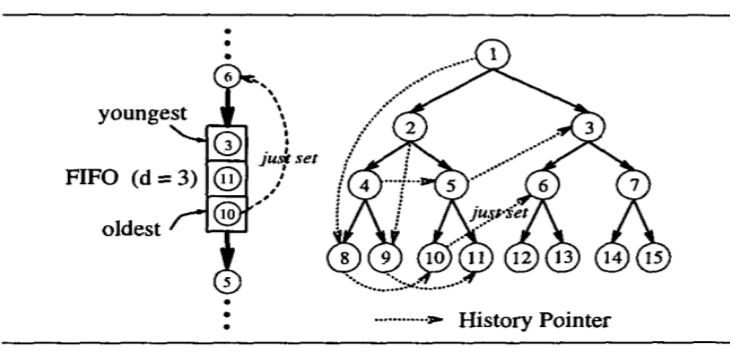
\epsfig{file=history.png,height=1.8in, width=3in}
\caption{Example showing the update of history-pointers}
\end{figure}
\subsubsection{Hardware Implementation}
To construct the history-pointers, we use  a FIFO queue
of length d which contains pointers to the last d nodes that have
just been visited. When we visit a new node $_hi$, the oldest node in
the queue will be $n_{i-d}$ (i.e. the node visited d nodes earlier), and
hence we update the history-pointer of $n_{i-d}$ to point to $h_i$. After
the first complete traversal of the LDS, all of the history-pointers
will be set. Figure 8 illustrates this process for the tree shown
earlier in Figure 4. Assuming that 
d = 3 and that we have just reached node 6, we would now update
the history-pointer of the oldest node in the 3-entry queue (node
10) to point to node 6, so we get a stride 3 pointer here.

\subsubsection{Evaluation}

Although history-pointer prefetching could improved latency tolerance
by accurate prefetching(flexible stride), it comes two additional 
forms of overhead: First, it needs to construct the history-pointers
which will need computation time, and sencond, it needs extra space to
store these new pointers which will cause cache miss too.
 
\subsection{Jump-Pointer Prefetching}
Roth et al. developed an effective Jump-Pointer Prefetching for Linked
Data Structures.\cite{Roth:1999:EJP:307338.300989}

\begin{figure*}
\centering
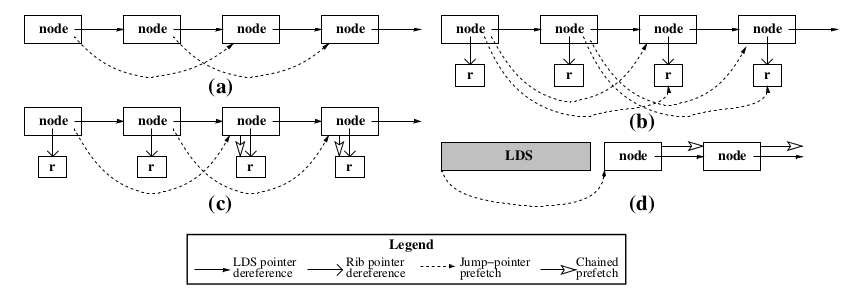
\epsfig{file=jump.png,height=1.8in, width=4in}
\caption{The four jump-pointer prefetching idioms. (a) Queue
  jumping. (b) Full jumping. (c) Chain jumping. (d) Root jumping.}
\end{figure*}

\subsubsection{Four prefetch idioms}
Roth et al. made a classification for Jump-Pointer here.
He divided Jump-Pointer into four different
idioms.\cite{Roth:1999:EJP:307338.300989} 

Queue jumping(Figure 9(a)) is the simplest idiom. Each node’s
jump-pointer points could  be accessed in the near future. The
distance between a node and the node pointed by its jump-pointer is 
called the jump interval, which is $||\mathcal{F}||$ exactly. As long
as this interval is large enough, 
the jump-pointer prefetching will 
complete before its corresponding demand access. 
But we could not access the first few nodes of queue jumping since no
Jump-Pointer pointing to them, this will cause stall time when
processor start to prefetch.

Full jumping(Figure 9(b)) is a variant of queue jumping for backbone-and-rib
structures, which consist of an LDS (backbone) with each node
containing one or more pointers to data 
nodes (ribs). Each node also has jump-pointers to the ribs of another
node, allowing ribs to be prefetched in parallel with the backbone. 

Chain jumping (Figure 9(c)) is a different method of prefetching rib
structures that does not include  the jump-pointers pointing to
ribs. The backbone of the LDS is 
prefetched using queue jumping, but the ribs 
are prefetched using natural pointers of the original data
structure which is also  called chained prefetches. Generally, the
processor issues chained 
prefetches from a node in the same iteration that it issues the
jump-pointer prefetch for the node. Therefore, if the jump-pointer
prefetch does not complete by the end of the iteration, the processor
will stall because of the address dependency for the chained prefetch. 
 
Root jumping(Figure 9(d)) is a variant of chained prefetching. It is
applicable to short LDS which are dominated by the 
startup period, it is also applicable to dynamic LDS where updating
jump pointers creates considerable overhead. In root
jumping, an entire LDS has a single jump-pointer to the next LDS to be
accessed. When an LDS traversal is begun, the jump pointer is used to
prefetch the first node of the next LDS. Subsequently, 
the natural pointers of the second LDS are used to issue prefetches to
its nodes in lockstep with the traversal of the first LDS. The use of
the natural pointers is like chained prefetching.

\subsubsection{Software Implementation}

JPP software implementations does not require extra hardware support,
it is completely implemented by modifying instruction, which could
make full use of the idiom classification mentioned above.

Roth et al. classifyed Olden benchmark suite into different idioms.
First, Bh, bisort, perimeter, power, treeadd, tsp and voronoi all
use “backbone-only” structures, so it is a good choice to make queue
jumping. For bisort and tsp, since both use large and extremely
volatile data structure, is hard to find a right idiom. Then em3d and
health  have “backbone-and ribs” structures, which can be taken as
full jumping and chain jumping. Finally mst which using dynamic list
is good to use root jumping.

After Roth et al. implemented the selected idiom(s) for each benchmark
by hand, they profiled the benchmarks to determine
which LDS loads contributed the majority of the cache
misses, and traced these back to their source level statements. Then
inserted the corresponding code for different idioms. It took about
one hour per benchmark to do these modification.
They only exploited knowledge of a program invariant
to streamline for mst when doing the jump-pointer creation
process. Given the uniformity of jump-pointer creation and
prefetching, jump-pointer prefetching can be automated in a 
compiler. 

\subsubsection{Cooperative Implementation}
From the classification of Jump-Pointer, we know that Jump-Pointer has
a strong connection with Chase-Pointer,Jump-pointer prefetches and
chained prefetches could be traded off for one another too, it even
could get an efficient prefetching solutions by combining them.  

Full jumping uses jump-pointer prefetches exclusively. At the other
hand,  root jumping uses few jump-pointer prefetches, and relies
heavily on Chase-Pointer prefetching. Chain jumping is somewhere in
the middle. Finally, queue jumping is a special 
case that handles simple structures using jump-pointer
prefetches only. So jump-pointer prefetching
and chained prefetching, can be implemented in either
hardware or software yielding four possible combinations.

Roth et al. presented a cooperative scheme in which jump-pointer
prefetching is done in software and chained prefetching is handled in
hardware. Although it is possible for software and hardware to
cooperate in reversed roles, this final combination 
makes little efficiency in terms of both complexity and performance.

\subsubsection{Evaluation}

\begin{figure}
\centering
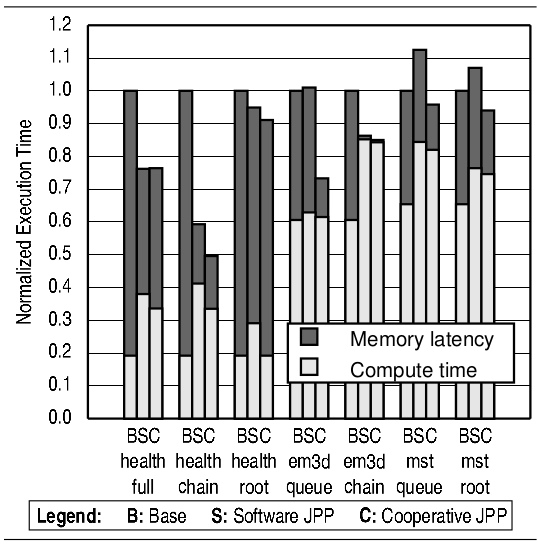
\epsfig{file=jpp.PNG,height=2.2in, width=3.2in}
\caption{Comparing idiom performance. Normalized
execution times of software and cooperative
implementations of the three prefetching
idioms.\cite{Roth:1999:EJP:307338.300989}} 
\end{figure}

Roth et al. evaluated the relative merits of the JPP idioms in the
context of the software and cooperative implementations.
They ignored hardware prefetching  because it implemented only one
idiom. Results are shown in Figure 10. 

Em3d, which is taken to be root jump, is costly to use jump queue and
Jump-Pointer to prefetch, consequently  an
algorithm that performs only explicit queue 
jumping in software and the array prefetches to be implemented in the
hardware is the most effective method here. 
Mst’s short hash table bucket chains are ideal for a root
jumping implementation. 
Although health’s dynamic lists
suggest root jumping, the lists are too long for this idiom
to be effective, chain jumping is the choice here.

From the Figure, we believe that  a combination
of jump-pointer prefetching for recurrent “backbone”
loads and chained prefetching for “rib” loads is the most
effective idiom. In the cooperative implementation, it can take
advantage of the automatic chained 
prefetching performed by the dependence hardware. 
Root jumping can be the most effective idiom in certain specialized
cases, in mst for instance, but is not a general purpose 
technique. Chain jumping is also the idiom implemented by the hardware
mechanism.
The result tells us that JPP is not applicable in every
situation. We need to adapte different algorithm according the data
features. 
 
\section{Content directed prefetching}

Cooksey et al. proposed Content-Directed Data Prefetching, a data
prefetching architecture that exploits the memory allocation used to
improve the performance of pointer-intensive applications constructed
by operating systems and runtime systems. This technique is developed
after conservative garbage collection, and prefetches potential virtual
addresses observed in memory references. This prefetching mechanism uses the
underlying data of the application, and provides an 11.3\% speedup
using no additionalprocessor state. By adding less than 1⁄2\% space
overhead to the second level cache, performance can be further
increased to 12.6\% across a range of real applications. 
\cite{Cooksey:2002:SCD:635506.605427}

\subsection{Basic CDP}

\subsubsection{Main idea}

The primary role of the prefetcher is to predict the  memory
accesses in a memory block which will be used in near future. The
content prefetcher attempts to predict future memory 
accesses by monitoring the memory traffic at a given level in the
memory hierarchy, looking directly for virtual addresses in the page
table. The prefetcher is based on the assumption that if a pointer 
is loaded from memory, there is a strong possibility that the address
will be used as the load address (effective address) of a future load.
Specifically, the content prefetcher works by examining the fill
contents of demand memory requests that have missed at some level in 
the memory hierarchy (e.g. L2 cache). When the fill request returns,
a copy of the cache line is passed to the content prefetcher, 
and the cache line is scanned for potential virtual addresses. If a
candidate address is found, a prefetch request is issued for that
address. The difficulty in this prediction technique is
trying to distinguish a virtual address from both data values and random bit
patterns.

\subsubsection{Hardware Implementation}

\begin{figure}
\centering
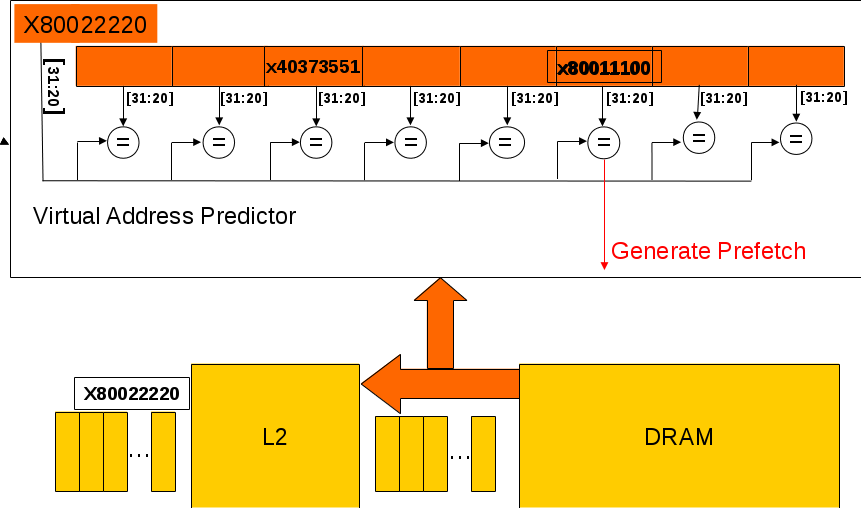
\epsfig{file=cdp.png,height=2.2in, width=3.2in}
\caption{CDP Hardware Implementation}
\end{figure}
From the Figure, the Predictor predict the target by the 3 bits of
virtal address, for example, the current virtual address is X80022220,
so the predictor will check the virtual address in the memory block if
there is an address matchs 800, and finally the virtual address
X80011100 becomes the prefetching target.

\subsubsection{Evaluation}
Although content-directed prefetching is attractive because it does
not care about the data flow, there is still a major deficiency in
its identification of addresses to 
prefetch. The intuition behind its choice
of candidate addresses is simple: if a pointer is loaded from memory,
there is a good likelihood that the pointer will be used as the data 
address of a future load. Unfortunately, this intuition results in a
significant deficiency: CDP generates prefetch requests for all
identified pointers in a scanned cache block. Greedily prefetching all
pointers results in low prefetch accuracy and significantly increases
bandwidth consumption and cache pollution  because not all loaded
pointers are later used as load addresses by the program. 
\begin{figure}
\centering
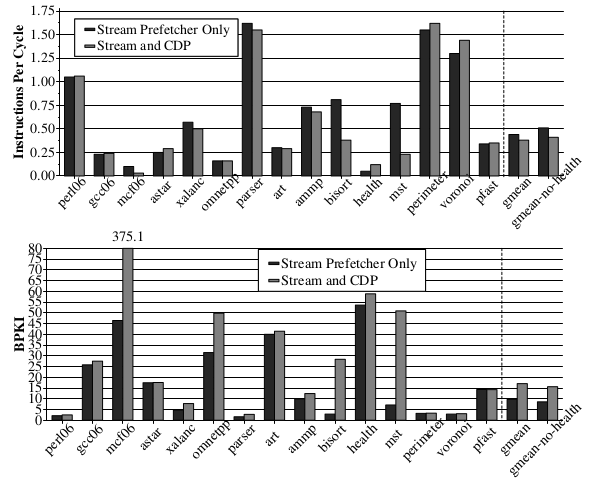
\epsfig{file=cdpdata.PNG,height=2.8in, width=3in}
\caption{Effect of the original CDP on performance and memory
  bandwidth\cite{4798232}} 
\end{figure}

Figure 12 shows the performance and bandwidth consumption (in terms
of BPKI-bus accesses per thousand retired instructions), 1) using
the baseline stream prefetcher alone, and 2) using both the baseline
stream prefetcher and CDP together.

 Adding CDP to a system with a stream prefetcher significantly reduces
 performance (by 4\%) and increases bandwidth consumption (by
 83.3\%). Even though 
CDP improves performance in several applications (gcc, astar,
health, perimeter, and voronoi), it still causes significant
performance loss and extra bandwidth consumption in several others
(mcf, xalancbmk, bisort, and mst). These effects are due to CDP’s
very low accuracy for these benchmarks, caused by indiscriminate
prefetching of all pointer addresses found in cache 
lines. Cache pollution resulting from useless prefetches is the major
reason why CDP degrades performance. 

\subsection{Enhanced Content Direct Prefetching }
Based on the research for CDP, especially for the low prefetch
accuracy problem, Ebrahimi et al. made some improvement, he added
two new components in this prefetching mechanism: 1) a compiler-guided
prefetch filtering mechanism which will choose more accurate load
address for hardware to prefetch. 2) a coordinated prefetcher
throttling mechanism that uses run-time feedback to manage the
interference between multiple  
prefetchers (LDS and stream-based) in a hybrid prefetching system. 
\cite{4798232}

\begin{figure}
\centering
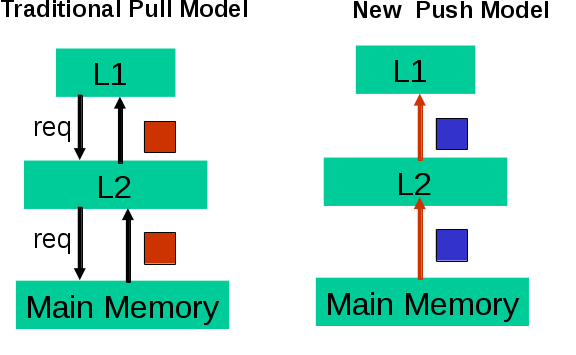
\epsfig{file=push.png,height=1.8in, width=2.4in}
\caption{Push vs Pull}
\end{figure}

\subsubsection{Implementation}

The first component  to efficient LDS prefetching in ECDP is
a compiler-guided technique that selectively identifies which pointer
addresses should be prefetched at run-time. The compiler uses its
knowledge of the location of pointers in LDS along with  the
usefulness of prefetches to determine which pointers would 
be beneficial to prefetch. The content-directed LDS prefetcher, at
run-time, uses this information to prefetch beneficial pointers instead of
indiscriminately prefetching all pointers.

Ebrahimi et al. use a profiling compiler to distinguish
beneficial and harmful PGs. The compiler profiles the code and
classifies each PG as harmful/beneficial based on the accuracy of the 
prefetches the PG generates in the profiling run. Using this
classification, the compiler provides hints to the content-directed
prefetcher. 
At runtime, the content-directed prefetcher uses these hints such that
it generates prefetch requests only for pointers in beneficial PGs.
To accomplish this, the compiler attributes a number of PGs to each
static load instruction.  During the profiling step, the compiler gathers
usefulness information about the PGs associated with each load
intruction in the program. The compiler informs the hardware of
beneficial PGs of each load using a hint bit vector. This bit vector
must be long enough to hold a bit for each possible pointer in a cache block.

At runtime, when a demand miss happens, the content-directed
prefetcher scans the fetched cache block and consults the missing
load’s hint bit vector. For a pointer found in the cache block, CDP
issues a prefetch request only if the bit vector indicates that
prefetching that pointer is beneficial. 


\section{Memory-side Prefetching}

All the research we talked above proposed to be processor-side
prefetching. More recently, Yang and Lebeck proposed prefetching
initiated near memory that we refer to as memory-side
prefetching.\cite{Yang:2002:PMH:646349.690705}
\cite{Hughes:2005:MPL:1066486.1066491} 
The difference between processor-side and memory-side prefetching
could be easlily foun through Figure 13. The usual processor-side
prefetching starts from the request from the processor, then pull the
right data from the memory, however memory-side prefetching does not
need the processor request, it push the data from memory directly
which could redecue the processor pressure when hiding the memory
latency. 

\begin{figure}
\centering
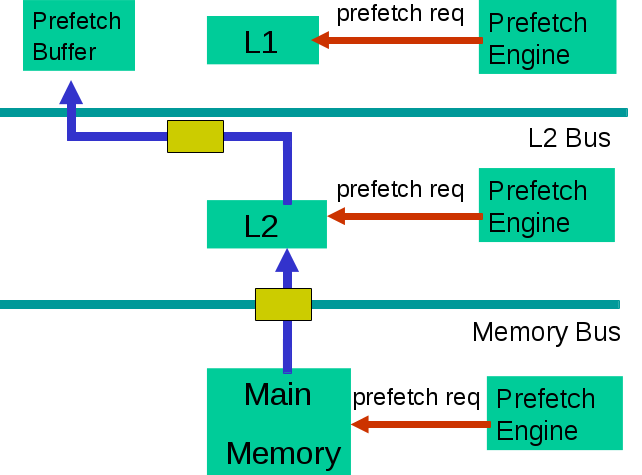
\epsfig{file=pushmodel.png,height=2in, width=2.4in}
\caption{Prefetch Engine}
\end{figure}

\subsection{Push-model Prefetching}

In this paper, Yang et al. proposed a cooperative hardware/software mechanism
to reduce memory access latencies for
LDSs.\cite{Yang:2002:PMH:646349.690705} Instead 
of relying on the past address history to predict future accesses,
they identify the load instructions that traverse the LDS, and execute
them ahead of the actual computation. 

In the push model, a controller-called a prefetch engine
is attached to each level of the memory hierarchy, as shown
in Figure 14. The prefetch engines (PFE) executes traversal kernels
independent of CPU execution. Cache blocks 
accessed by the prefetch engines in the L2 or main memory levels are
pushed up to the CPU and stored either in 
the L1 cache or a prefetch buffer. The prefetch buffer is
a small, fully-associative cache, which can be accessed in
parallel with the L1 cache. The remainder of this section
describes the design details of this novel push architecture.

\begin{figure}
\centering
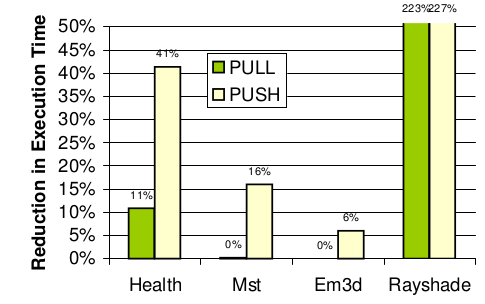
\epsfig{file=pushdata.PNG,height=2in, width=2.4in}
\caption{Push vs. Pull: Macrobenchmark Results.\cite{Yang:2002:PMH:646349.690705}}
\end{figure}

\subsubsection{Evaluation}
Figure 15 shows the speedup for both push and pull 
prefetching using our benchmarks on systems that incur a 
one cycle overhead for address translation with a perfect 
TLB. From Figure 10 we could see that the push model outperforms the
pull model for all four benchmarks. Rayshade  
shows the largest benefits, with speedups of 227\% for the 
push model, and 223\% for the pull model. Health achieves 
41\% improvement in execution time for the push model 
while achieving only 11\% for the pull model. Similarly, for 
the push model, em3d and mst achieve 6\% and 16\%, respectively, while
neither shows any benefits by using the pull model.  

\begin{figure*}
\centering
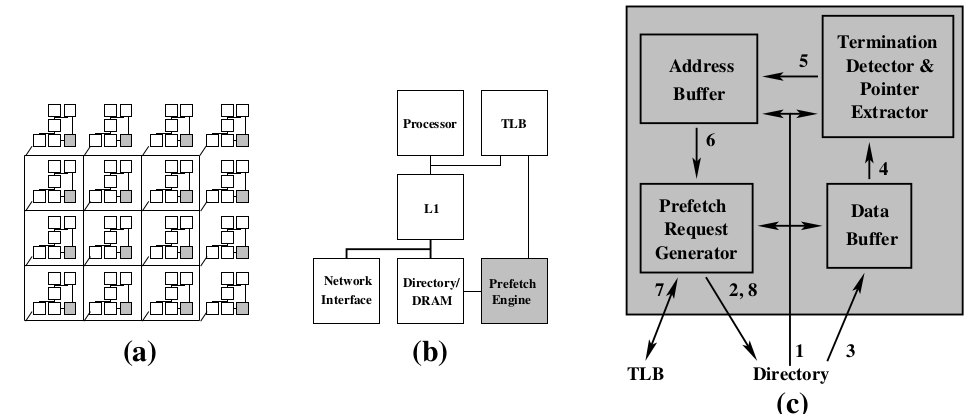
\epsfig{file=pim.PNG,height=1.8in, width=4.8in}
\caption{A PIM with a prefetching engine in a multi-PIM system. (a)
  The multi-PIM system. 
(b) The contents of the PIM. The prefetch engine is highlighted. (c)
The contents of the prefetch engine, along with the steps to prefetch an LDS.}
\end{figure*}

\subsection{PIM Prefetching}


Hughes et al. provided a memory-side scheme here, The scheme consists
of a prefetch engine close to memory that can speculate on LDS data
that a processor may need from that memory, a software command from
the requesting processor encodes a summary of the LDS and the expected
traversal. The prefetch engine uses the command to execute the
traversal seperately, requesting memory to send the traversed data to the
processor. Although the prefetch engine’s traversal is also
serialized, its proximity to memory results in faster service than
requests initiated at the processor. This potentially allows the
prefetch engine to run ahead of the processor, initiating data
transfers earlier than the processor and pipelining multiple
transfers over the network.\cite{Hughes:2005:MPL:1066486.1066491}

\subsubsection{Implementation}
The base architecture is a multiprocessor built solely from 
multiple PIM chips (Figure 16 (a)).The PIMs are connected 
to each other via a conventional multiprocessor network in a
directory-based, cache-coherent, release consistent shared-memory
organization. Using a common model of a
multiprocessor node for the PIM, place all of 
the components on the same chip (Figure 16(b)).

The key part of the memory-side prefetching system is a prefetch
engine on each PIM chip. The engine workes next to the directory and
communicates only 
through it, but also accesses the 
processor’s TLB (Figure 16(b)).The engine prefetches data from the
adjacent memory for all processors in the system. The hardware for the 
prefetch engine is minor relative to that 
for a state-of-the-art processor, consisting of only a few buffers, a
counter, some comparators, multiplexors, 
decoders, and some straightforward control logic.

The purpose of the prefetch engine is to traverse an LDS ahead of the
processor and send the data to the processor 
before its corresponding demand access, like pushing the data from
memory to processor. 
This requires information about the LDS structure and traversal 
path. A general way to convey this information is  to
send to the prefetch engine code that 
can be executed to traverse the LDS for the processor, and for the
prefetch engine to have the ability to execute such code.
 

In practice, the LDS traversal path depends primarily 
on the LDS structure and sometimes on the results of simple
comparisons involving the data within the LDS. 
Further, the LDS structure and the comparison operations can often be
encoded concisely in a few bytes. 
Therefore,  we assume special prefetch commands that encode this
information, and require the programmer or compiler to insert such
commands in the code before an LDS traversal. 

The mechanism supports three common LDS types – linked lists, trees,
and “backbone and rib structures”, also support depth-first,
breadth-first, and some non-deterministic traversals. So Hughes et
al. implemented the prefetch command that encodes the LDS
traversals. The command is not intended to be universally applicable, 
but to strike a good balance between flexibility and prefetch engine complexity.
The command consists of the op code and the address of the first node
of the LDS to be traversed . 

A processor issuing a prefetch command sends it to the directory of
the node that contains the first LDS node to be traversed. The actions
required to process the command and the various components of the prefetch 
engine are illustrated in Figure 16(c) and discussed next.

Basicly, the PIM mechanism here useas a prefeth engine and some
special commend to finish the LDS traversal.

\begin{figure*}
\centering
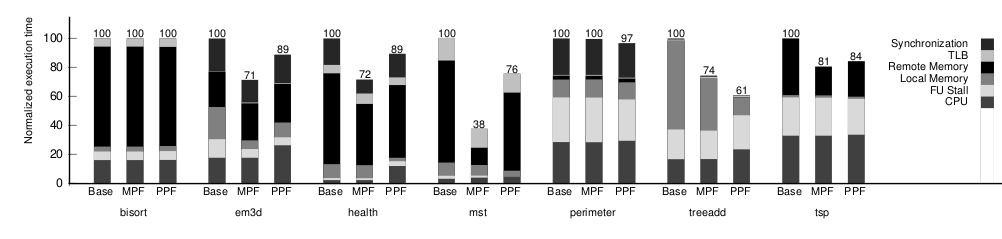
\epsfig{file=pimdata.PNG,height=1.6in, width=4.8in}
\caption{Normalized execution times. Results for base system (Base), memory-side
prefetching (MPF), and processor-side (software jump-pointer)
prefetching (PPF)..\cite{Hughes:2005:MPL:1066486.1066491}} 
\end{figure*}

\subsubsection{Evaluation}

Figure 17 shows that five of the benchmarks see significant
improvements in performance from MPF (19\% 
to 62\%), while the other two, bisort and perimeter, shows an
insignificant change. The average reduction in 
execution time over the six benchmarks with significant LDS stall time
(i.e., excluding perimeter) is 27\%. 
Bisort and perimeter do not show any benefits because their traversal
paths cannot be exactly captured by the implemented prefetch command
and so very few prefetches could be inserted. The traversal paths of
the other five benchmarks can be captured by the implemented prefetch 
command, and they perform significant improvements. 

\section{Related work}


\subsection{Multi-Chain Prefetching\cite{Choi:2004:GFP:986533.986536}}

While pointer-chasing is inherently sequential, pointer-chasing
computations typically traverse multiple pointer chains in an
independent fashion. Such independent pointer-chasing traversals
represent a large source of memory parallelism. Choi et al. explores
the possibility of exploiting such memory  parallelism for the
purposes of memory latency tolerance by presenting a memory
scheduling algorithm that computes a prefetch schedule from an LDS
traversal  and  a prefetch engine architecture capable of traversing
LDSs.  Finally, they conduct an experimental evaluation of
prefetching technique on 
four pointer-chasing applications. The results show multi-chain
prefetching increases performance between 52\% and 78\%. 

\subsection{Prefetch Array Prefetching\cite{824351}} 
Recently, Karlsson et al. proposed a technique to reduce the startup
stall time for jump-pointer prefetching. This technique creates an
array of pointers, called the prefetch array, pointing to the first few nodes 
in an LDS that do not have jump-pointers. Just before accessing the
LDS, prefetches are issued to all nodes 
pointed by the prefetch array, potentially hiding some latency for
those nodes as well.
 They implemented prefetch arrays for the relevant benchmarks. With jump-pointer
prefetching and prefetch arrays, health sees 
a 20\% reduction in execution time over the base system (as opposed to
11\% with jump-pointers but without 
prefetch arrays and 29\% with memory-side prefetching). The other
benchmarks showed or are expected to 
show little benefit over jump-pointer prefetching without prefetch
arrays or even some performance degradation. Overall, we found that the prefetch
arrays technique did not give consistent 
benefits over the jump-pointer prefetching schemes of Roth and Sohi,
but has potential for hiding startup 
stall time in some cases.

\subsection{Guidded Region
  Prefetching\cite{Wang:2003:GRP:871656.859663}} 

In this paper, Wang et al. proposed a cooperative hardware-software
 prefetching scheme called Guided Region Prefetching (GRP), Guided
 Region Prefetching (GRP) uses static compiler analysis to produce a
 set of load hints for its 
hardware prefetching engine, which includes the original CDP scheme
[9]. GRP is a coarse-grained mechanism: it enables or disables
prefetching for all pointers 
in cache blocks fetched by a load instruction. 

\section{Summary}

Four kinds of prefetching techniques for LDS have been
proposed in this paper. 

The first two kinds of technique focus on the data patterns of LDS,
it includes Chase-Pointer and Jump-Pointer Prefetch, these two
prefetching could be seen as fine-grain prefetching.
Amir and Luk most contributed to this prefetching.
Amir's Dependence-based prefetching and Luk's Greedy prefetching
belong to the Chase-Pointer problem while their Jump-Pointer
prefetching and History-Pointer prefetching belong to Jump-Pointer
problem. \cite{Roth:1999:EJP:307338.300989}\cite{Roth:1998:DBP:384265.291034}\cite{Luk:1996:CPR:248208.237190}  

The third prefetching technique is based on mointering high-level
memory traffic insead of anlysising the state of data flow, it is a
coarse-grain prefetching, Cooksey's CDP and Ebrahimi's ECDP belong to
this classification.\cite{Cooksey:2002:SCD:635506.605427}\cite{4798232}

The last one  uses an opposite perspective, not like the first three
which need the processor to pull the prefetching data, it will push
the data from memory directly by processor in memory. Yang and Hughes
did the most work in this
part. \cite{Yang:2002:PMH:646349.690705}\cite{Hughes:2005:MPL:1066486.1066491} 

All of these approachs offer an good performance
to hide memory latency than base system without prefetching technique,
a cooperate approach combined Jump-Pointer software and Chase-Pointer
hardware implementation make an impressive result during the data
analysis approach. Although CDP approach only does well for part of
applications , its simple idea and hardware implementation still leave
a huge development space. Memory side prefetching becomes available
as the showing up of processor in memory (PIM), and gives a better
parallelism implementation. 

%\end{document}  % This is where a 'short' article might terminate

%ACKNOWLEDGMENTS are optional

\section{Acknowledgments}

This is a research paper for class CS5431, also comes with a presentation.
%
% The following two commands are all you need in the
% initial runs of your .tex file to
% produce the bibliography for the citations in your paper.
\bibliographystyle{abbrv}
\bibliography{sigproc}  % sigproc.bib is the name of the Bibliography in this case
% You must have a proper ".bib" file
%  and remember to run:
% latex bibtex latex latex
% to resolve all references
%
% ACM needs 'a single self-contained file'!
%
%APPENDICES are optional
%\balancecolumns

\balancecolumns
% That's all folks!
\end{document}
